% atomic.tex
\documentclass{beamer}
\usetheme{Warsaw}
\author{Aditya Patawari, Lalatendu Mohanty}
\institute{
  Contributor to Fedora Project and Project Atomic\\[2ex]
  \texttt{aditya@adityapatawari.com}\\
  \texttt{lmohanty@redhat.com}\\
  \texttt{adimania, lalatenduM on freenode irc}\\
  \texttt{http://blog.adityapatawari.com}
}
\title{Running your containers in a sane environment, Project Atomic}
\usepackage{graphicx}
\usepackage{ragged2e}
\usepackage{fancyvrb}
\usepackage[free-standing-units, space-before-unit, use-xspace]{siunitx}
\begin{document}

\begin{frame}
  \titlepage
  \end{frame}
\begin{frame}{Topics}
\begin{itemize}
  \item What is the problem?
  \item How Docker helps?
  \item Why not LXC containers or VM?
  \item Project Atomic is here!
  \item .. Along with some components
  \item Starting our Atomic Host
  \item Demo
\end{itemize}
\end{frame}

\begin{frame}{What is the problem?}
\begin{figure}[htp]
\centering

\includegraphics[scale=0.15]{problem.jpg}
\label{}
\end{figure}
\begin{itemize}
  \item My production needs to be homogeneous
  \item I need to ship entire environment to my colleague
  \item I need a stable environment to run containers
  \item I need to support automation
  \item Managing hosts should involve minimal efforts
\end{itemize}
\end{frame}

\begin{frame}{How Docker helps?}
\begin{figure}[htp]
\centering

\includegraphics[scale=0.30]{docker_logo.png}
\label{}
\end{figure}
\begin{itemize}
  \item Lightweight linux container
  \item Boots up in seconds
  \item Incrementally build, revert and reuse your container
  \item API to manage things remotely
\end{itemize}
\end{frame}

\begin{frame}{Why not LXC containers or VM?}
\begin{figure}[htp]
\centering

\includegraphics[scale=0.15]{fight.png}
\label{}
\end{figure}
\begin{itemize}
  \item Less resource consuming than virtual machines
  \item Faster than VM with reasonable amount of isolation. According to a benchmark by Boden Russell, IBM (approx figures):
  \begin{itemize}
    \item CPU usage 20\percent vs 70\percent
    \item Memory usage 50 MB vs 300 MB
  \end{itemize}    
  \item Better tools ecosystem around docker than LXC
  \item Case study of Spotify
\end{itemize}
\end{frame}

\begin{frame}{Project Atomic is here!}
\begin{figure}[htp]
\centering

\includegraphics[scale=0.25]{atomic_logo.png}
\label{}
\end{figure}
\begin{itemize}
  \item It is not a new GNU/Linux distribution
  \item Framework to create an OS from RHEL, CentOS or Fedora
  \item Aim of Project Atomic is to create a better OS for containers
\end{itemize}
\end{frame}

\begin{frame}{Why Project Atomic?}
\begin{figure}[htp]
\centering

\includegraphics[scale=0.25]{atomic_logo.png}
\label{}
\end{figure}
\begin{itemize}
  \item Minimal operating system (Less packages to maintain)
  \item Optimized operating system for containers
  \item Benefits of our favorite Enterprise Linux
  \item Robust atomic upgrades
  \item More secure than traditional operating systems.
\end{itemize}
\end{frame}

\begin{frame}{What Atomic Hosts Won't Provide?}
\begin{itemize}
  \item Yum/dnf install/update will not work in Atomic host
  \item Official CentOS/Fedora/RHEL images would have minimal package set
\end{itemize}
\end{frame}

\begin{frame}{Atomic hosts comprises of}
\begin{itemize}
  \item rpm-ostree
  \item systemd
  \item Cockpit
  \item Kubernetes
  \item /usr/bin/atomic
  \item Docker
  \item SPC
\end{itemize}
\end{frame}

\begin{frame}{rpm-ostree}
\begin{figure}[htp]
\centering

\includegraphics[scale=0.70]{Rpm_logo.png}
\label{}
\end{figure}
\begin{itemize}
  \item Git for operating systems
  \item Atomic upgrade and rollbacks
  \item Derived from GNOME OSTree project.
  \item Bootable, immutable, versioned filesystem trees
\end{itemize}
\end{frame}

\begin{frame}{Why rpm-ostree?}
\begin{figure}[htp]
\centering
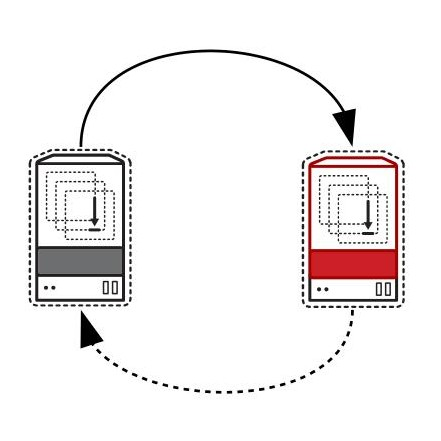
\includegraphics[scale=0.25]{ostree.jpg}
\label{}
\end{figure}
\begin{itemize}
  \item Composed from standard rpms
  \item No need to re-invent the wheel on packaging
  \item No more half way upgraded systems
  \item Option to rollback to previous state (old good state).
\end{itemize}
\end{frame}

\begin{frame}{How rpm-ostree works?}
\begin{itemize}
  \item Only /etc and /var are writable
  \item All data (e.g. containers) are unchanged on upgrade
  \item /etc gets updated through a 3-way merge
\end{itemize}
\end{frame}

\begin{frame}{Systemd}
\begin{figure}[htp]
\centering

\includegraphics[scale=0.45]{systemd.png}
\label{}
\end{figure}
\begin{itemize}
  \item System and service manager for Linux 
  \item Replacing the init in Centos 7
  \item Highly modular and much more powerful than sysV
  \item Check out http://0pointer.de/blog/projects/why.html
\end{itemize}
\end{frame}

\begin{frame}{..Introducing Cockpit..}
\begin{figure}[htp]
\centering
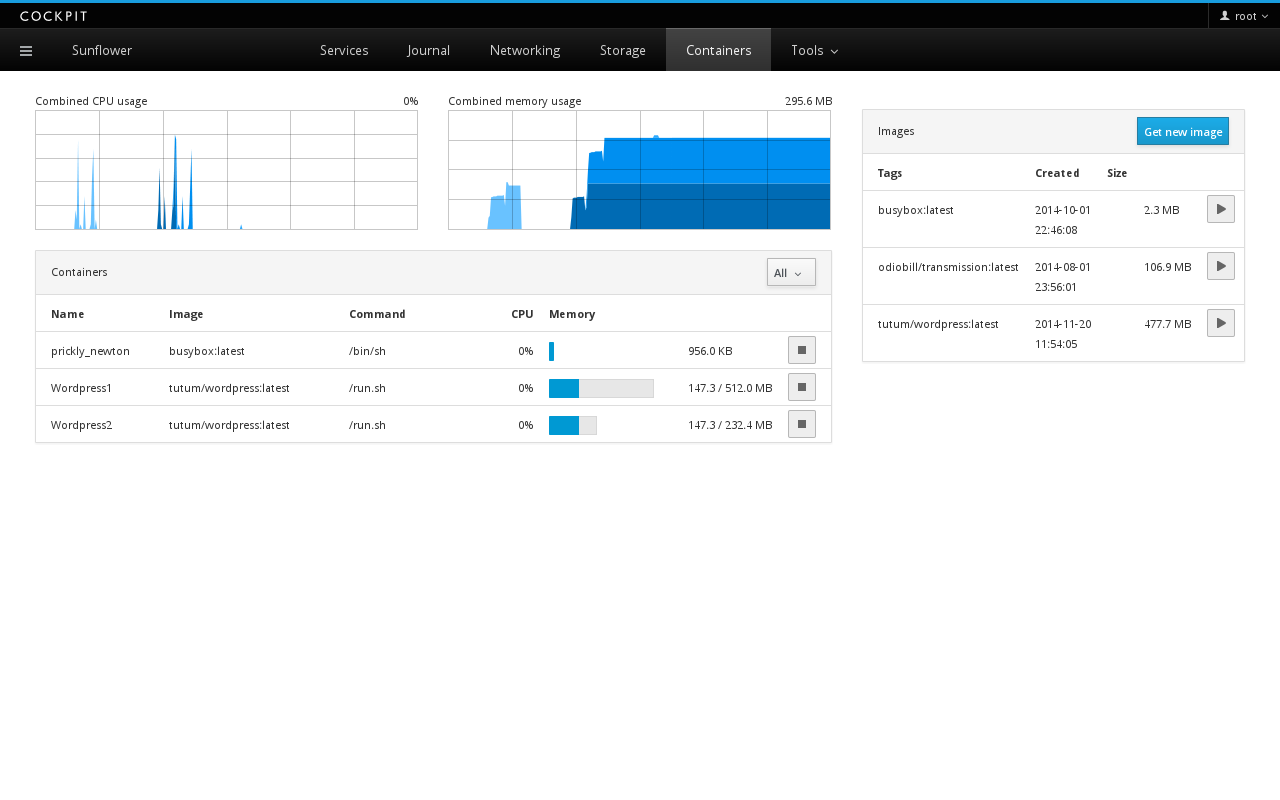
\includegraphics[scale=0.28]{cockpit.png}
\label{}
\end{figure}
\end{frame}

\begin{frame}{..Kubernetes ..}
\begin{figure}[htp]
\centering

\includegraphics[scale=0.2]{kubernetes.png}
\label{}
\end{figure}
\begin{itemize}
  \item Master-slave arch
  \item For managing containerized applications across multiple hosts
  \item It gives basic mechanisms for deployment, maintenance, and scaling of applications.
  \item Lots of examples and setup instructions at https://github.com/GoogleCloudPlatform/kubernetes
\end{itemize}
\end{frame}

\begin{frame}{/usr/bin/atomic}
\begin{itemize}
  \item Coherent entry point : manage host and containers with the atomic command
  \item Fill gaps in Linux container implementations.
  \item “atomic install foo” can install a container with its k8s configuration and/or systemd unit file
  \item “atomic run” grabs the LABEL “run” with its all command line details.
  \item It can use/serve the metadata for containers for different use cases
\end{itemize}
\end{frame}

\begin{frame}{SPC}
\begin{itemize}
  \item SPC = Super Privileged Containers
  \item Debugging tools, monitoring tools etc as container images
  \item Runs with --privileged option
\end{itemize}
\end{frame}

\begin{frame}{Projects For Multi-container Applications}
\begin{itemize}
  \item Nulecule  - https://github.com/projectatomic/nulecule
  \item Atomicapp - https://github.com/projectatomic/atomicapp
\end{itemize}
\end{frame}

\begin{frame}{Introducing Nulecule}
\begin{figure}[htp]
\centering
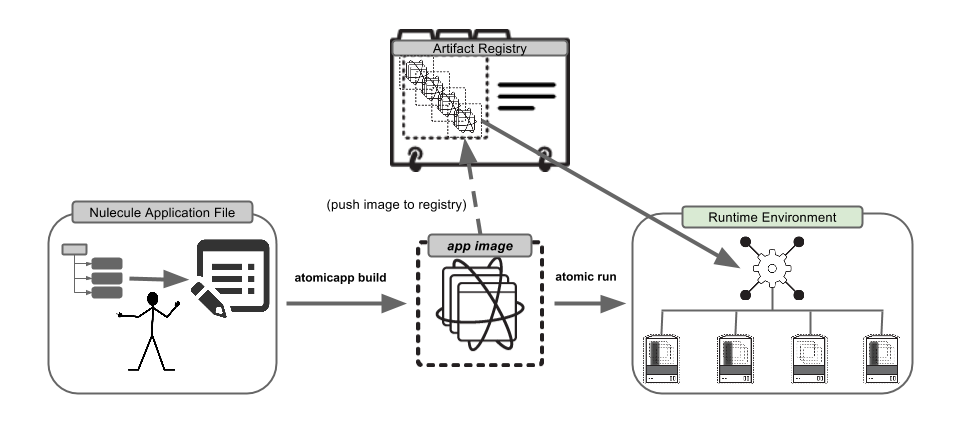
\includegraphics[scale=0.25]{nulecule.png}
\label{}
\end{figure}
\begin{itemize}
  \item Composite Container-based Application Specification
  \item Provide a simple, flexible way to describe a multi-container application, including all dependencies
  \item Package once. Run anywhere*
\end{itemize}
\end{frame}

\begin{frame}{.. And Atomicapp}
\begin{itemize}
  \item Atomicapp is a reference implementation of the Nulecule Specification
  \item It can be used to bootstrap container applications and to install and run them
  \item Atomicapp is designed to be run in a container context
\end{itemize}
\end{frame}

\begin{frame}{Demo!}
\begin{figure}[htp]
\centering

\includegraphics[scale=0.40]{demo.jpg}
\label{}
\end{figure}
\begin{itemize}
  \item Start a container.
  \item Verify that it works.
  \item Kill the container.
  \item OOOOO... Magic!
\end{itemize}
\end{frame}


\begin{frame}{Questions?}
Now is your chance :)
\end{frame}

\end{document}
